
%(BEGIN_QUESTION)
% Copyright 2007, Tony R. Kuphaldt, released under the Creative Commons Attribution License (v 1.0)
% This means you may do almost anything with this work of mine, so long as you give me proper credit

Which of these tubes will generate the most hydrostatic pressure, assuming they all contain the same type of liquid at precisely the same (vertical) height?

$$\includegraphics[height=7cm]{i02953x01.eps}$$

\underbar{file i02953}
%(END_QUESTION)





%(BEGIN_ANSWER)

This is a ``trick'' question: they all generate the exact same amount of hydrostatic pressure.

\vskip 10pt

The principle at work here is the relationship between {\it vertical} height and hydrostatic pressure.  Cross-sectional area of the liquid column is irrelevant!  Only column height, liquid density, and the gravitational pull of the Earth matter when calculating hydrostatic pressure.  Since all three of these variables are precisely the same in this scenario, the hydrostatic pressures must likewise be precisely the same.

%(END_ANSWER)





%(BEGIN_NOTES)


%INDEX% Physics, static fluids: hydrostatic pressure

%(END_NOTES)


